%% --------------------------------------------------------------
%%
%% R E S U L T S
%%
%% --------------------------------------------------------------

\section{Preliminary Results}
\subsection{Modelling sGRB afterglow (GRB170817A)}
\begin{frame}{}  %% ---------- Intro/motivation 
    \begin{tikzpicture}[overlay,remember picture]
        \uncover<1->{ % <-> |
            \node (t1) [anchor=center,scale=1,opacity=1] at ([shift={(-3.0cm,2.5cm)}]current page.center){
                \parbox{0.7\textwidth}{
                    \begin{itemize}
                        \item Gaussian jet $E(\theta) \propto e^{(\theta/\theta_c)^2}$
                        \item Off-axis $\theta_{\rm obs} > \theta_c$
                        \item Relativistic core, $\Gamma_c \sim 10^2$; low ISM density.
                    \end{itemize}
            }};
        }
        \uncover<1->{ % <-> |
            \node (img1) [anchor=center,scale=1,opacity=1] at ([shift={(1.cm,-1.35cm)}]current page.center){
                \parbox{1.0\textwidth}{
                    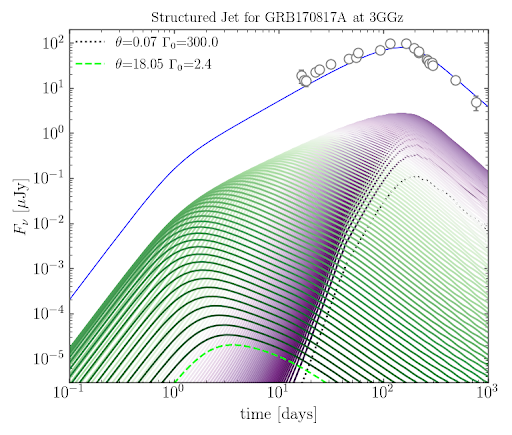
\includegraphics[height=6cm]{figures/grb170817fernandezPyBlastAfterglow.png}
            }};
        }
        \uncover<1->{ % <-> |
            \node (img1) [anchor=center,scale=1,opacity=1] at ([shift={(9.0cm,-0.5cm)}]current page.center){
                \parbox{1.0\textwidth}{
                    Flux centroid motion, $4.5\,$GGz; \\
                    Color is $I/I_{\rm max}$ %is shown with $I=0.01I_{\rm max}$ cut
                    
                    \movie[width=0.8\textwidth]{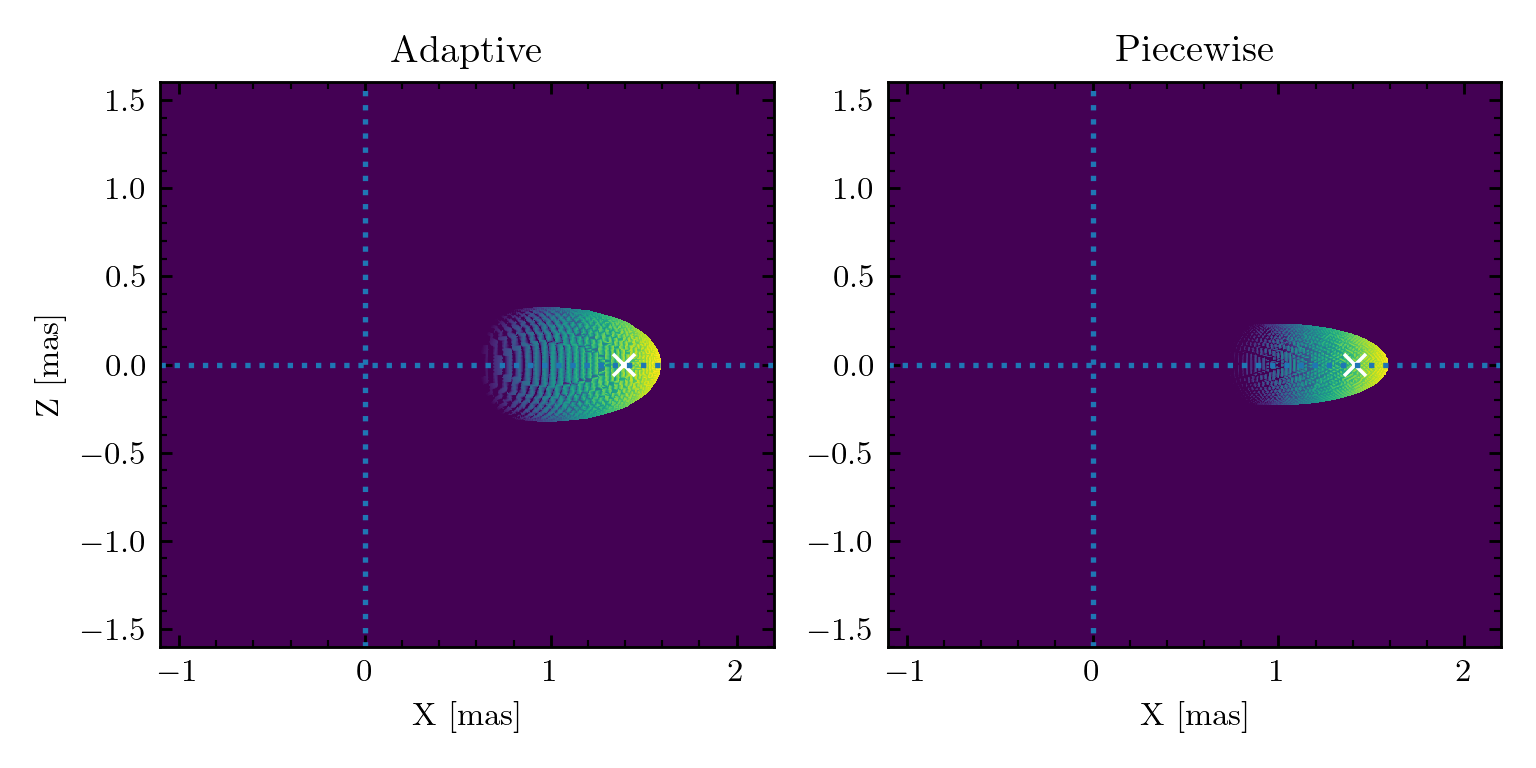
\includegraphics[width=0.8\textwidth]{figures/200.png}}{figures/out2.mp4}
            }};
        }
    \end{tikzpicture}
\end{frame}


% =============================================================================================

\subsection{Kilonova afterglow for NR ejecta profiles}
\begin{frame}{}  %% ---------- Intro/motivation 
    \begin{tikzpicture}[overlay,remember picture]
        \uncover<1->{ % <-> |
            \node (t1) [anchor=center,scale=1,opacity=1] at ([shift={(-3.1cm,-0.5cm)}]current page.center){
                \parbox{0.65\textwidth}{
                    %                    \textbf{Main Features}:
                    \begin{itemize}
                        \item Set of NS BNS simulations targeted to \GW{}.
                        %
                        \item BNS model $(q,\tilde{\Lambda})$ $q=M_A/M_B$ is the mass ratio, $\tilde{\Lambda}$ tidal deformability parameter (Depends in EOS of NS)
                        %
                        \item Ejecta $M,\beta,E_k = f(q,\tilde{\Lambda})$
                        %
                    \end{itemize}
                    
                    \textbf{Assuming that GRB170817A change in afterglow is due to the emergence of a new component}: 
                    \begin{itemize}
                        \item New way to constrain binary parameters, EOS
                        %
                        \item Additional information on ISM
                        %
                        \item Information on shock physics
                        %
                    \end{itemize}
            }};
        }
        \uncover<1-1>{ % <-> |
            \node (img1) [anchor=center,scale=1,opacity=1] at ([shift={(5.0cm,1.8cm)}]current page.center){
                \parbox{0.5\textwidth}{
                    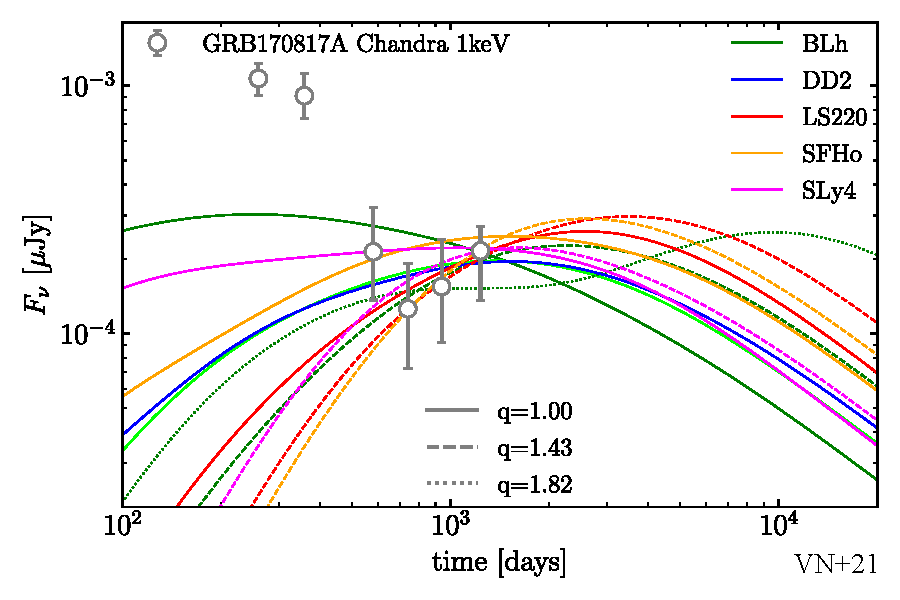
\includegraphics[height=3.8cm]{figures/best_xray_obs_representative_all_eos.pdf}
                    
                    %\small{\textbf{Artist depiction of ejecta$^\text{\citep{Ascenzi:2020xqi}}$}}
            }};
        }
        \uncover<1-1>{ % <-> |
            \node (img1) [anchor=center,scale=1,opacity=1] at ([shift={(5.2cm,-2.2cm)}]current page.center){
                \parbox{0.5\textwidth}{
                    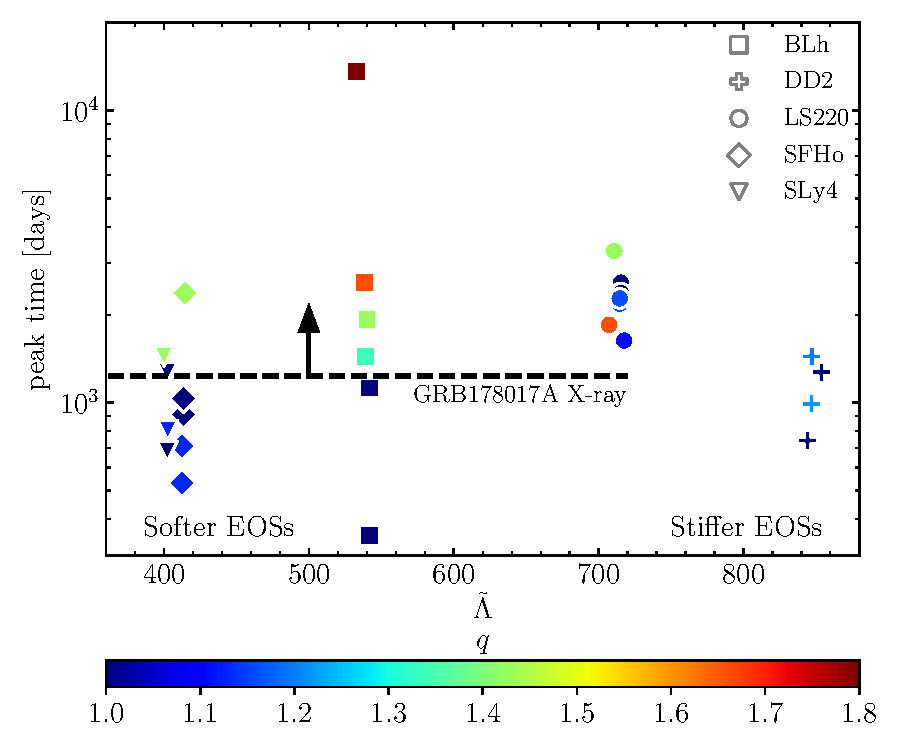
\includegraphics[height=4.2cm]{figures/scatter_lightcurve_tpeak_vs_lambda.pdf}
                    
                    %\small{\textbf{Artist depiction of ejecta$^\text{\citep{Ascenzi:2020xqi}}$}}
            }};
        }
    \end{tikzpicture}
\end{frame}

% =============================================================================================

\subsection{Thermal electrons in mildly relativistic shocks}
\begin{frame}{}  %% ---------- Intro/motivation 
    \begin{tikzpicture}[overlay,remember picture]
        \uncover<1->{ % <-> |
            \node (t1) [anchor=center,scale=1,opacity=1] at ([shift={(-3.0cm,2.2cm)}]current page.center){
                \parbox{0.5\textwidth}{
                    \begin{itemize}
                        \item ``Thermal spectrum'' (left)
                        \item ``Non-thermal spectrum'' (right)
                    \end{itemize}
                    $\beta_{\rm sh}=0.1$, $n_{\rm ISM}=10^4\,\ccm$, $t=200\,$d, $\delta=0.1$, $p=3$, $B=0.1\,$G, $\varepsilon_T=0.1$
            }};
        }
        \uncover<1->{ % <-> |
            \node (t1) [anchor=center,scale=1,opacity=1] at ([shift={(4.0cm,2.2cm)}]current page.center){
                \parbox{0.5\textwidth}{
                    \begin{eqnarray*}
                        \frac{\partial N}{\partial \gamma}\Big|_{\rm th} &= n_{e} \frac{ \gamma^2\sqrt{1-\gamma^{-2}} }{K_2(1/\Theta) \Theta} e^{-\gamma/\Theta}, \\
                        %                        \hspace{5mm}
                        \frac{\partial N}{\partial \gamma}\Big|_{\rm pl} &= n_e g(\Theta)\delta\frac{p-2}{3\Theta}\Big(\frac{\gamma}{3\Theta}\Big)^{-p}
                    \end{eqnarray*}
                    
                    
                    %                    Spectrum $3$ segments: 
                    %                    (i) $\nu < \nu_c$: low energy tail, $F_{\nu}\propto\nu^{1/3}$, 
                    %                    (ii) $\nu(\gamma) > \nu_c$ power law segment $F_{\nu}\propto\nu^{-1/2}$ 
                    %                    (iii) $\nu(\gamma)$and 
            }};
        }
        \uncover<1->{ % <-> |
            \node (img1) [anchor=center,scale=1,opacity=1] at ([shift={(2.cm,-1.5cm)}]current page.center){
                \parbox{1.0\textwidth}{
                    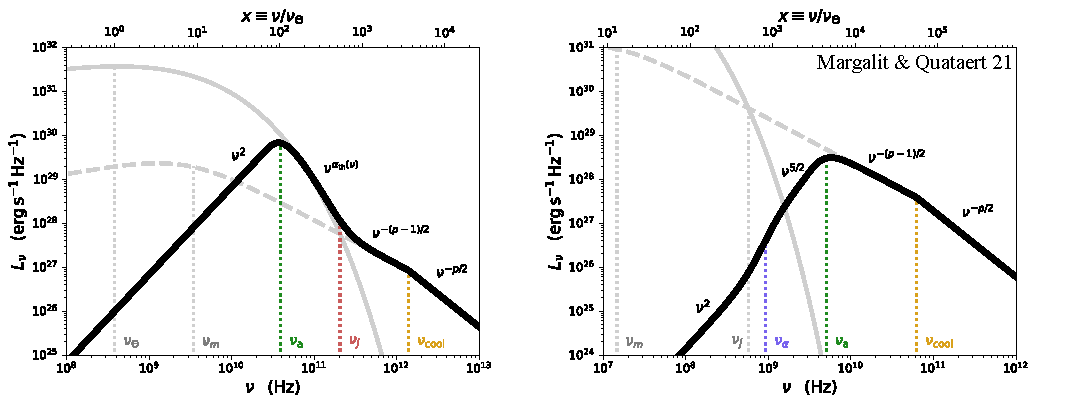
\includegraphics[height=5cm]{figures/Margalit21_thermalElectrons.pdf}
            }};
        }
    \end{tikzpicture}
\end{frame}
\begin{frame}{}  %% ---------- Intro/motivation 
    \begin{tikzpicture}[overlay,remember picture]
        \uncover<1->{ % <-> |
            \node (t1) [anchor=center,scale=1,opacity=1] at ([shift={(-5.0cm,1.2cm)}]current page.center){
                \parbox{0.4\textwidth}{
                    Comparison between two optically thin ight cruves:
                    \begin{itemize}
                        \item ``Thermal'' (blue)
                        \item ``Non-thermal'' (green)
                    \end{itemize}
                    Further investigations required! 
            }};
        }
        \uncover<1->{ % <-> |
            \node (img1) [anchor=center,scale=1,opacity=1] at ([shift={(6.cm,0.0cm)}]current page.center){
                \parbox{1.0\textwidth}{
                    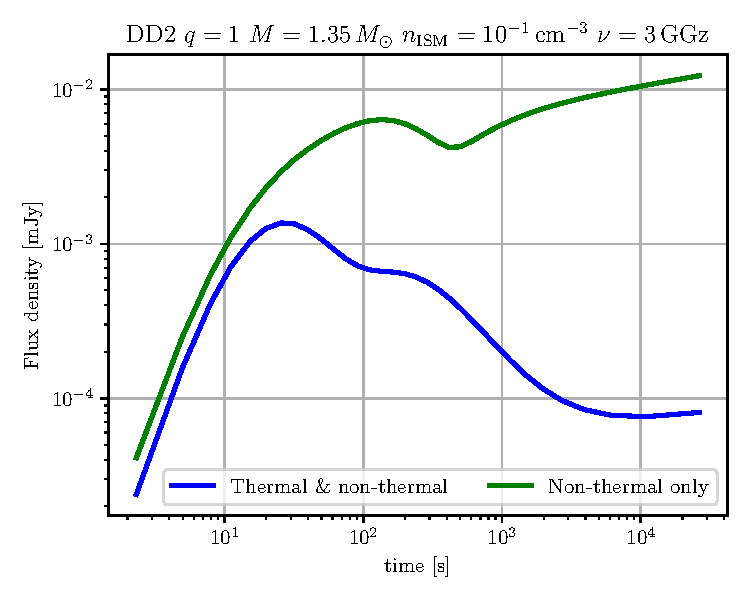
\includegraphics[height=7cm]{figures/test_thermal_electrons.pdf}
            }};
        }
    \end{tikzpicture}
\end{frame}

% =============================================================================================

\subsection{Extracting kilonova ejecta profile}
\begin{frame}{}  %% ---------- Intro/motivation 
    \begin{tikzpicture}[overlay,remember picture]
        \uncover<1->{ % <-> |
            \node (t1) [anchor=center,scale=1,opacity=1] at ([shift={(-3.0cm,2.5cm)}]current page.center){
                \parbox{0.7\textwidth}{
                    \begin{itemize}
                        \item $E_{\rm k} = f(\theta,\beta)$
                        \item $E_{\rm k;max}$ at $\theta\rightarrow0$ and $\beta\rightarrow0.2$.
                        \item $\log_{10}(E_k)=b_0 + (b_1 \theta) + (b_2 \beta) + (b_3 \theta^2) + (b_4 \theta \beta) + (b_5 \beta^{1/4})$
                    \end{itemize}
            }};
        }
        \uncover<1->{ % <-> |
            \node (img1) [anchor=center,scale=1,opacity=1] at ([shift={(2.2cm,-1.35cm)}]current page.center){
                \parbox{1.0\textwidth}{
                    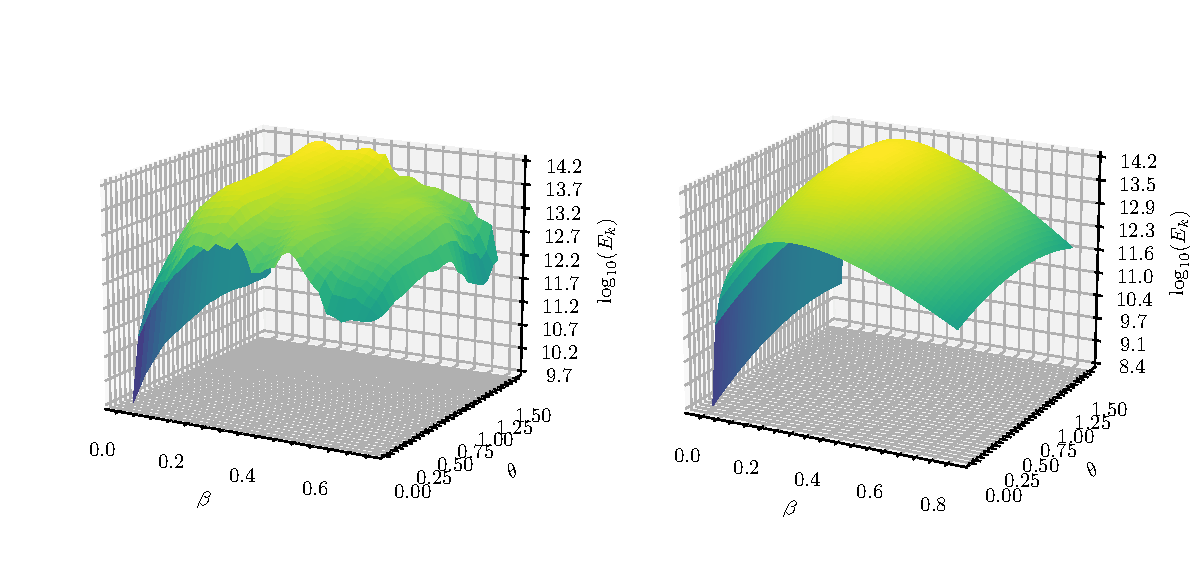
\includegraphics[height=6cm]{figures/fit_2d_ejecta.pdf}
            }};
        }
        \uncover<1->{ % <-> |
            \node (img1) [anchor=center,scale=1,opacity=1] at ([shift={(9cm,2cm)}]current page.center){
                \parbox{1.0\textwidth}{
                    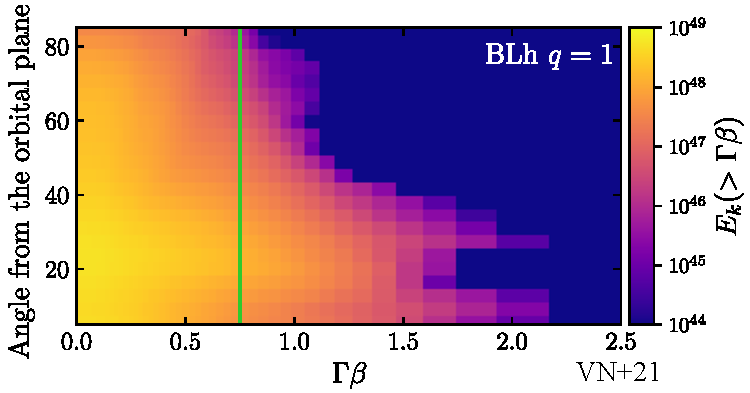
\includegraphics[height=3cm]{figures/kinetic_energy_struct_models_bottom_only.pdf}
            }};
        }
    \end{tikzpicture}
\end{frame}

% =============================================================================================

\subsection{Dynamics in the toy model}
\begin{frame}{}  %% ---------- Intro/motivation 
    \begin{tikzpicture}[overlay,remember picture]
        \uncover<1->{ % <-> |
            \node (t1) [anchor=center,scale=1,opacity=1] at ([shift={(-4.8cm,1.2cm)}]current page.center){
                \parbox{0.45\textwidth}{
                    kN ejecta expands into ISM 'processed' by GRB
                    Three possible scenaria 
                    \begin{itemize}
                        \item kN ejecta behind \& inside the GRB one
                        \item kN ejecta behind \& outside the GRB one
                        \item kn ejecta ahead of the GRB one
                    \end{itemize}
                    Further investigations required! 
            }};
        }
        
        \uncover<2->{ % <-> |
            \node (t1) [anchor=center,scale=1,opacity=1] at ([shift={(-4.8cm,-2.6cm)}]current page.center){
                \parbox{0.45\textwidth}{
                    \textcolor{red}{Error!} 
                    Shells $\Gamma_{\rm jet} = \Gamma_{\rm ej}$ at $R_{\rm jet}=R_{\rm ej}$ 
                    at \textbf{different} times.
                    
                    Consier a toy model 
                    ($1$ ejectan and $1$ jet spherical shell)
            }};
        }
        
        \uncover<1->{ % <-> |
            \node (img1) [anchor=center,scale=1,opacity=1] at ([shift={(6.cm,0.0cm)}]current page.center){
                \parbox{1.0\textwidth}{
                    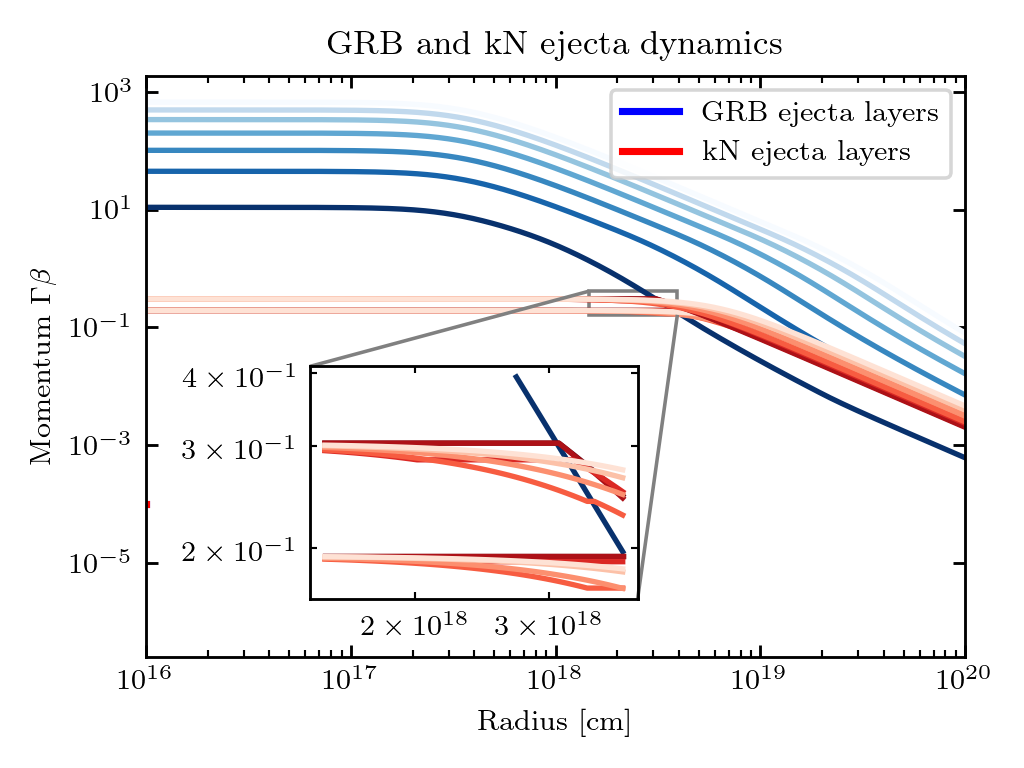
\includegraphics[height=7cm]{figures/plot_pretty_dynamics.png}
            }};
        }
    \end{tikzpicture}
\end{frame}

% =============================================================================================

\subsection{Dynamics in the toy model [Incl. density behind slowed GRB BW]}
\begin{frame}{}  %% ---------- Intro/motivation 
    \begin{tikzpicture}[overlay,remember picture]
        \uncover<1-1>{ % <-> |
            \node (t1) [anchor=center,scale=1,opacity=1] at ([shift={(-4.8cm,2.2cm)}]current page.center){
                \parbox{0.42\textwidth}{
                    Improving shell interaction
                    \begin{itemize}
                        \item $dU/dR\rightarrow dU/dt_b$ where $U\in\{R,\Gamma,E_{\rm int}...\}$, $t_b$ is time in burster frame. Shell "collide" at $t_{\rm coll}$, $R_{\rm jet} = R_{\rm ej}$. 
                    \end{itemize}
            }};
        }
        \uncover<1-1>{ % <-> |
        \node (t1) [anchor=center,scale=1,opacity=1] at ([shift={(-4.8cm,-2.2cm)}]current page.center){
            \parbox{0.42\textwidth}{
                What happens at shell collision?
        }};
        } 
        \uncover<3-5>{ % <-> |
        \node (t1) [anchor=center,scale=1,opacity=1] at ([shift={(-4.8cm,1.2cm)}]current page.center){
            \parbox{0.42\textwidth}{
                Improving shell interaction
                \begin{itemize}
                    \item $dU/dR\rightarrow dU/dt_b$ where $U\in\{R,\Gamma,E_{\rm int}...\}$, $t_b$ is time in burster frame. Shell "collide" at $t_{\rm coll}$, $R_{\rm jet} = R_{\rm ej}$. 
                    \item Behind the BW $\rho$ is low but $\rho\neq0$. Consider Taylor-von Neumann-Sedov BW. 
                \end{itemize}
        }};
        }
        \uncover<1-1>{ % <-> |
            \node (img1) [anchor=center,scale=1,opacity=1] at ([shift={(5.0cm,0.0cm)}]current page.center){
                \parbox{1.0\textwidth}{
                    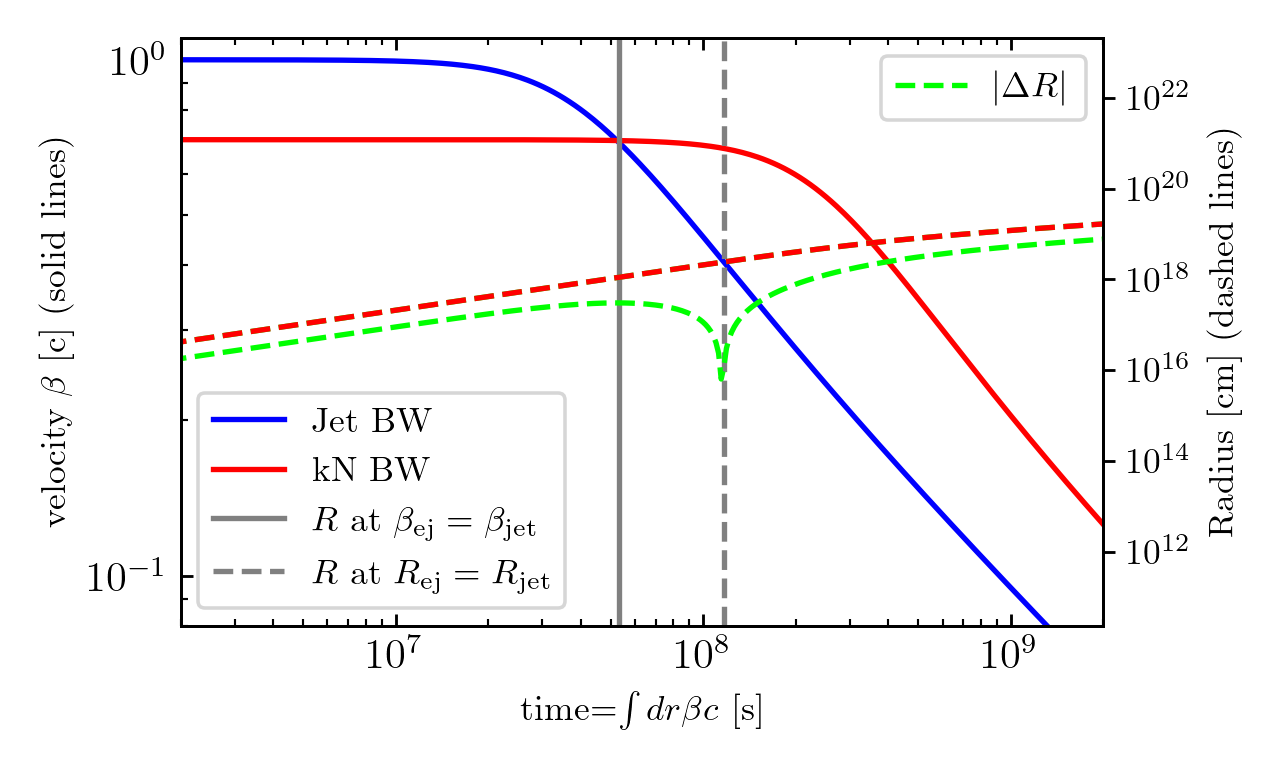
\includegraphics[height=6.0cm]{figures/time_intersection.png}
            }};
        }
        \uncover<2-2>{ % <-> |
            \node (t1) [anchor=center,scale=1,opacity=1] at ([shift={(0.0cm,-0.2cm)}]current page.center){
                \parbox{0.80\textwidth}{
                    What happens at collision of shells?
                    \begin{eqnarray*}
                        T^{\mu\nu} &=& (\rho' c^2 + \omega' p')u^{\mu}u^{\nu} + p'\eta^{\mu\nu} \\
                        E_{\rm tot} &=& \int{T^{00}}dV = \Gamma m + \Gamma_{\rm eff}(\hat{\gamma})E_{\rm int}'\\
                        P^{i} &=& c\sqrt{\Gamma^2 - 1} (m + \hat{\gamma}E_{\rm int}' / c^2 ) 
                    \end{eqnarray*}
                    Energy and momentum conservation at the collision of $2$ shells:
                    \begin{eqnarray*}
                        E_{\rm tot; f} &=& E_{\rm tot; 1} + E_{\rm tot; 2} \\
                        P_{\rm f} &=& P_{1} + P_{2}
                    \end{eqnarray*}
                    Non-linear system of equations that gives the 
                    initial state, $\Gamma_f$ and $E_{\rm int;f }'$  of the 'merged' shell.
                    
                    \textcolor{green}{Possible for two simple shells} \\
                    \textcolor{red}{Impossible for structured\&spreading shells -- Dead End}
            }};
        }
        \uncover<3-3>{ % <-> |
            \node (img1) [anchor=center,scale=1,opacity=1] at ([shift={(5.0cm,0.0cm)}]current page.center){
                \parbox{1.0\textwidth}{
                    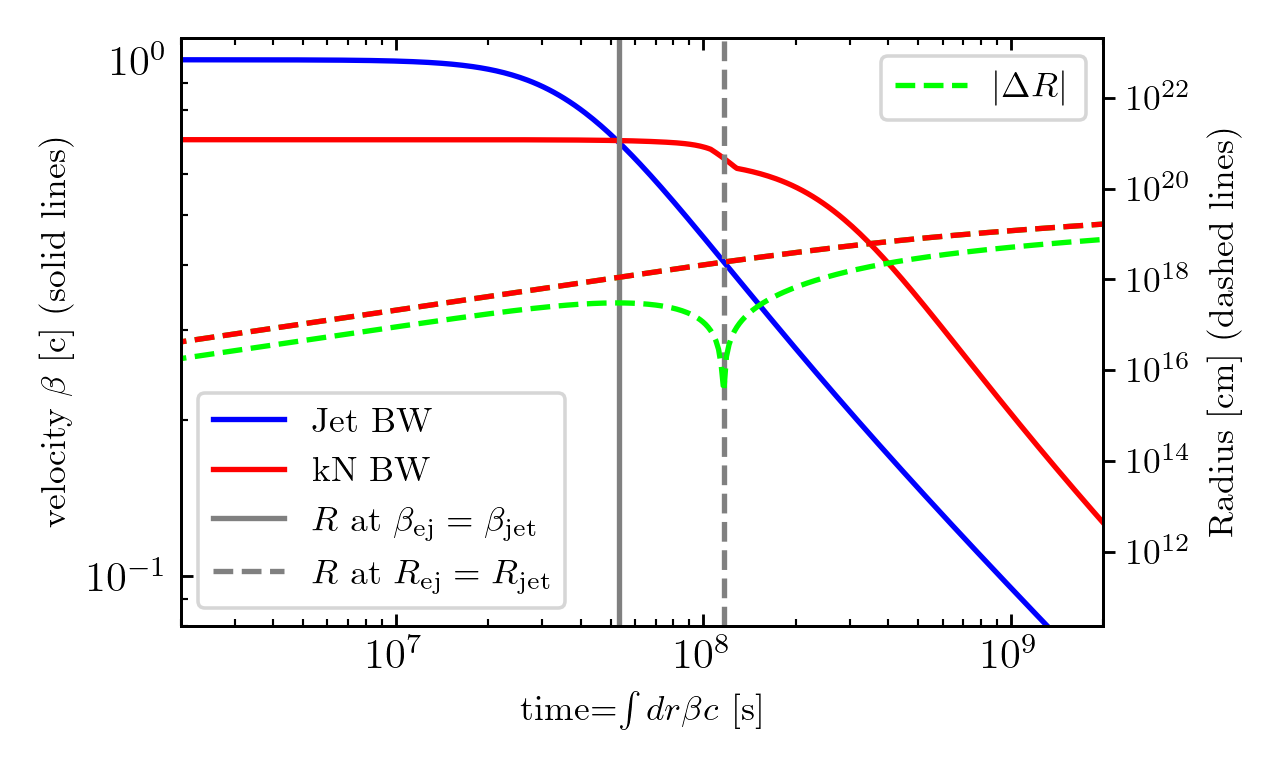
\includegraphics[height=6.0cm]{figures/time_intersection2.png}
            }};
        }
        
        
        \uncover<4-4>{ % <-> |
        \node (img1) [anchor=center,scale=1,opacity=1] at ([shift={(5.0cm,0.1cm)}]current page.center){
            \parbox{1.0\textwidth}{
                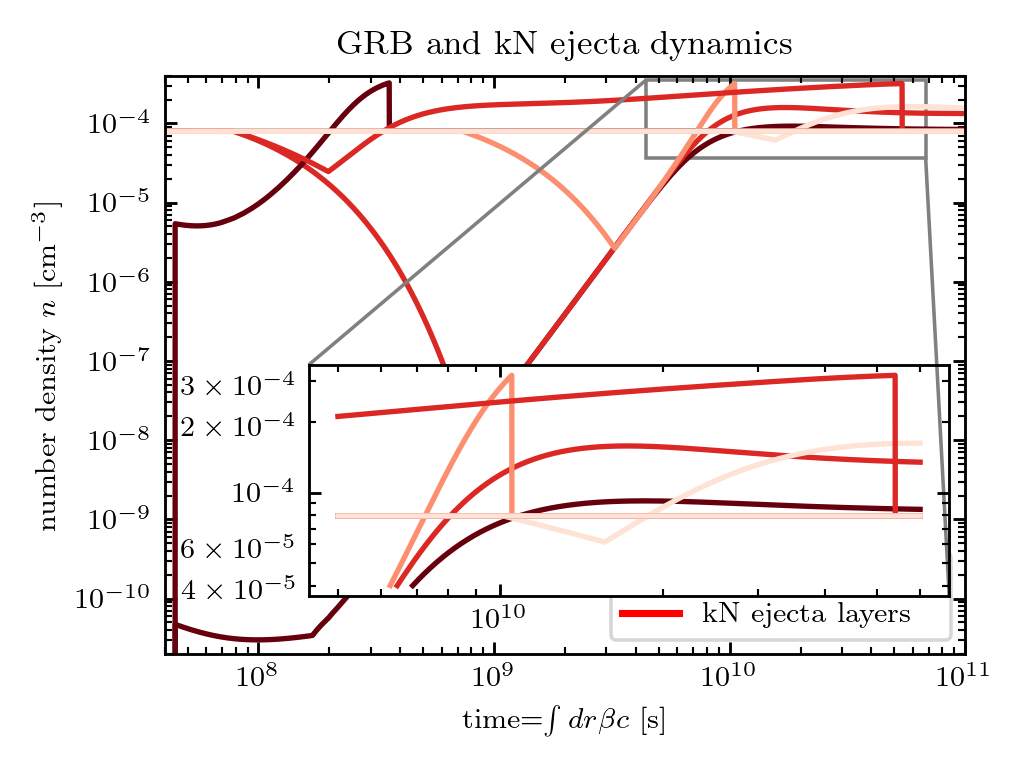
\includegraphics[height=7.0cm]{figures/plot_pretty_dynamics_rho_full.png}
        }};
        }
        \uncover<5-5>{ % <-> |
            \node (img1) [anchor=center,scale=1,opacity=1] at ([shift={(5.0cm,0.1cm)}]current page.center){
                \parbox{1.0\textwidth}{
                    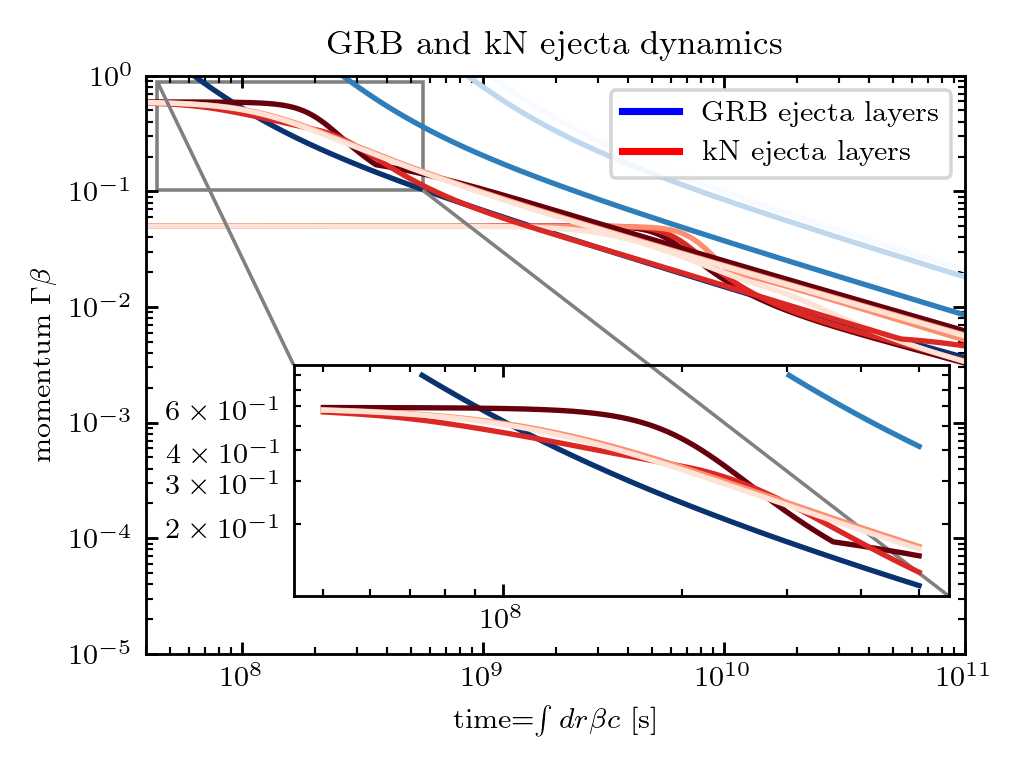
\includegraphics[height=7.0cm]{figures/plot_pretty_dynamics_full.png}
            }};
        }
        \uncover<3-5>{ % <-> |
        \node (img1) [anchor=center,scale=1,opacity=1] at ([shift={(-0.0cm,-2.4cm)}]current page.center){
            \parbox{1.0\textwidth}{
                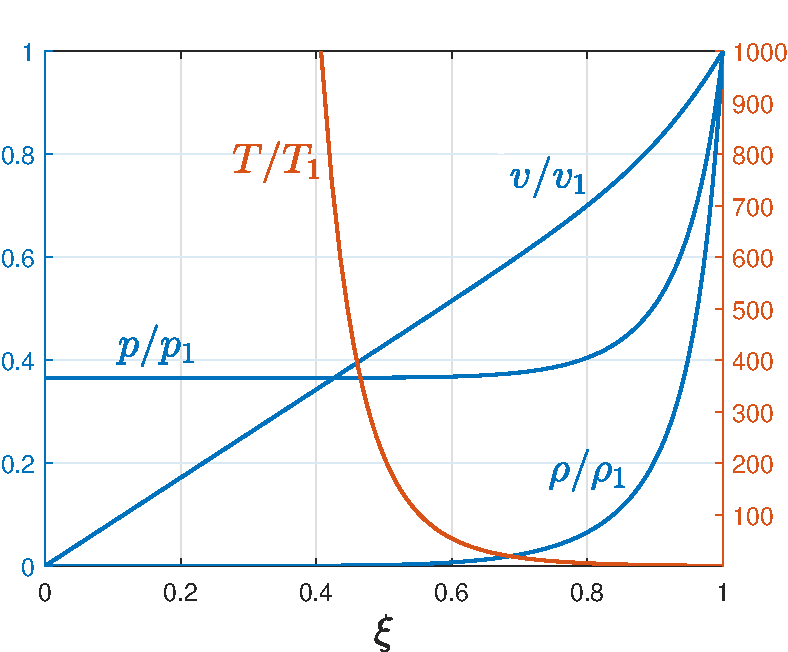
\includegraphics[height=3.5cm]{figures/TNS_blast_wave.pdf}
        }};
    
        }
        \uncover<3-3>{ % <-> |
        \node (t1) [anchor=center,scale=1,opacity=1] at ([shift={(3.5cm,-3.6cm)}]current page.center){
            \parbox{0.60\textwidth}{
                \textcolor{red}{Major code change: jet and ejecta BWs have to solved together}.
        }};
        }
        \uncover<4-4>{ % <-> |
        \node (t1) [anchor=center,scale=1,opacity=1] at ([shift={(3.5cm,-3.6cm)}]current page.center){
            \parbox{0.60\textwidth}{
                \textcolor{green}{Major code change: jet and ejecta BWs have to solved together}.
        }};
        }
        \uncover<5-5>{ % <-> |
            \node (t1) [anchor=center,scale=1,opacity=1] at ([shift={(3.5cm,-3.6cm)}]current page.center){
                \parbox{0.60\textwidth}{
                    \textcolor{orange}{Missing: effect of the realtive vlocity $\beta_{12}=\frac{\beta_1 - \beta_2}{1 - \beta_1\beta_2}$}.
            }};
        }
        \uncover<6-6>{ % <-> |
        \node (t1) [anchor=center,scale=1,opacity=1] at ([shift={(-1.0cm,-0.0cm)}]current page.center){
            \parbox{0.99\textwidth}{
                Derive dynamics of a fluid expanding in a non-uniform, pre-accelerate ISM
                \begin{equation*}
                    \begin{aligned}
                        T^{\mu\nu} =& (\rho' c^2 + e' p')u^{\mu}u^{\nu} + p'\eta^{\mu\nu}, \, p' = (\hat{\gamma}-1)(e'- \rho' c^2), \, E_{\rm int} = (e' - \rho'c^2)V' \\ 
                        E_{\rm tot} =& \int{T^{00}}dV = \Big(\Gamma^2\rho' c^2 + (\hat{\gamma}\Gamma^2-\hat{\gamma}+1)e'\Big) \frac{V'}{\Gamma} = \Gamma m + \Gamma_{\rm eff}(\hat{\gamma})E_{\rm int}'\\
                        dE_{\rm tot} =& 0 \rightarrow d [ \Gamma (M_0 + m) c^2 + \Gamma_{\rm eff}E_{\rm int}' ] = \Gamma_{\rm ISM} dm c^2 + \Gamma_{\rm eff} dE_{\rm rad}' \\
                        dE_{\rm int} =& dE_{\rm sh} + dE_{\rm ad} + dE_{\rm rad} \\
                        dE_{\rm sh} =& (\Gamma_{\rm rel}-1) dm c^2, \, \Gamma_{\rm rel} = \Gamma\Gamma_{\rm ISM}(1-\beta\beta_{\rm ISM}\rm) \\
                        dE_{\rm ad} =& - p dV + TdS = -(\hat{\gamma}-1)(E_{\rm int}'/V') dV' = -(\hat{\gamma}-1)E_{\rm int}' d\ln V' \\
%                        V' \propto R^3 \Gamma_{\rm ISM} / \Gamma_{\rm rel}; \\
%                        d\ln V' =& d\ln m - d\ln\rho - d\ln\Gamma_{\rm rel} + d\ln\Gamma_{\rm ISM}\\
                        \frac{d\Gamma}{dR} &= \frac{ -(\Gamma-\Gamma_{\rm ISM} + \Gamma_{\rm eff} (\Gamma_{\rm rel}-1)) + \Gamma_{\rm eff}(\hat{\gamma}-1)E_{\rm int}' \Big( \frac{dm}{dR}\frac{1}{m} - 
                        \textcolor{red}{\frac{d\rho_{\rm ISM}}{dR}}\frac{1}{\rho_{\rm ISM}} -
                        \textcolor{red}{\frac{d\Gamma_{\rm ISM}}{dR}}\frac{1}{\Gamma_{\rm ISM}} \Big) }{ (M_0 + m)c^2 + \frac{d\Gamma_{\rm eff}}{d\Gamma}E_{\rm int}' + \Gamma_{\rm eff}(\hat{\gamma}-1)E_{\rm int}' 
                        \textcolor{red}{\frac{d\Gamma_{\rm rel}}{d\Gamma}}\frac{1}{\Gamma_{\rm rel}} },
                    \end{aligned}
                \end{equation*}
%                \begin{eqnarray*}
%                    T^{\mu\nu} &=& (\rho' c^2 + \omega' p')u^{\mu}u^{\nu} + p'\eta^{\mu\nu} \\
%                    E_{\rm tot} &=& \int{T^{00}}dV = \Gamma m + \Gamma_{\rm eff}(\hat{\gamma})E_{\rm int}'\\
%                    P^{i} &=& c\sqrt{\Gamma^2 - 1} (m + \hat{\gamma}E_{\rm int}' / c^2 ) 
%                \end{eqnarray*}
%                Energy and momentum conservation at the collision of $2$ shells:
%                \begin{eqnarray*}
%                    E_{\rm tot; f} &=& E_{\rm tot; 1} + E_{\rm tot; 2} \\
%                    P_{\rm f} &=& P_{1} + P_{2}
%                \end{eqnarray*}
%                Non-linear system of equations that gives the 
%                initial state, $\Gamma_f$ and $E_{\rm int;f }'$  of the 'merged' shell.
%                
%                \textcolor{green}{Possible for two simple shells} \\
%                \textcolor{red}{Impossible for structured\&spreading shells -- Dead End}
        }};
    }
    \end{tikzpicture}
\end{frame}

% =============================================================================================

\subsection{Complex shell dynamics}
\begin{frame}{}  %% ---------- Intro/motivation 
    \begin{tikzpicture}[overlay,remember picture]
        \uncover<1->{ % <-> |
            \node (t1) [anchor=center,scale=1,opacity=1] at ([shift={(-4.5cm,1.2cm)}]current page.center){
                \parbox{0.45\textwidth}{
                    Dynamics of the kilonova ejecta, 
                    shaped by the GRB jet \\ 
                    
                    Left two panels: \\
                    Interaction with slowest GRB layer \\
                    
                    Right two panels: \\
                    Interaction with fastest GRB layer
                    
                    Top panels: 
                    
                    
            }};
        }
        \uncover<1->{ % <-> |
            \node (img1) [anchor=center,scale=1,opacity=1] at ([shift={(6.1cm,1.7cm)}]current page.center){
                \parbox{1.0\textwidth}{
                    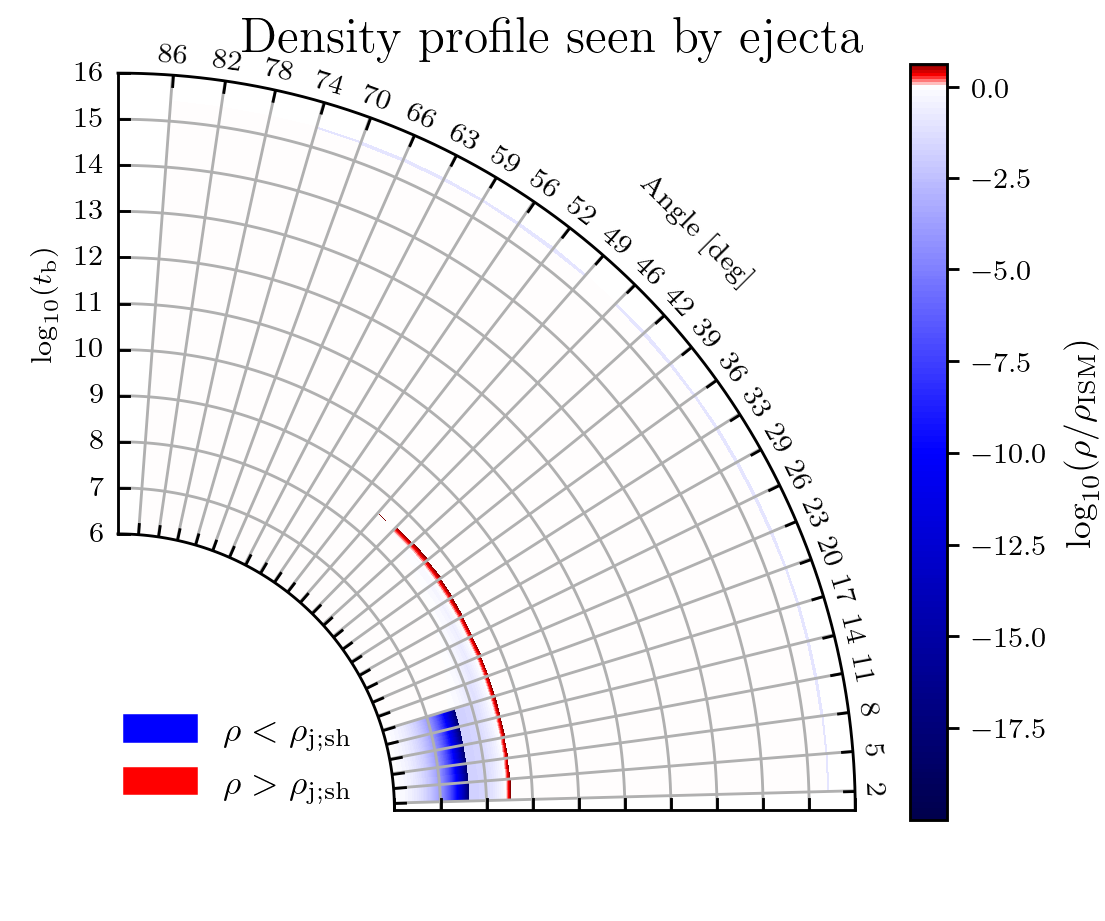
\includegraphics[height=4cm]{figures/bw_ej_dens_ism_evol_slow_shell_2.png}
            }};
        }
        \uncover<1->{ % <-> |
            \node (img1) [anchor=center,scale=1,opacity=1] at ([shift={(6.1cm,-2.3cm)}]current page.center){
                \parbox{1.0\textwidth}{
                    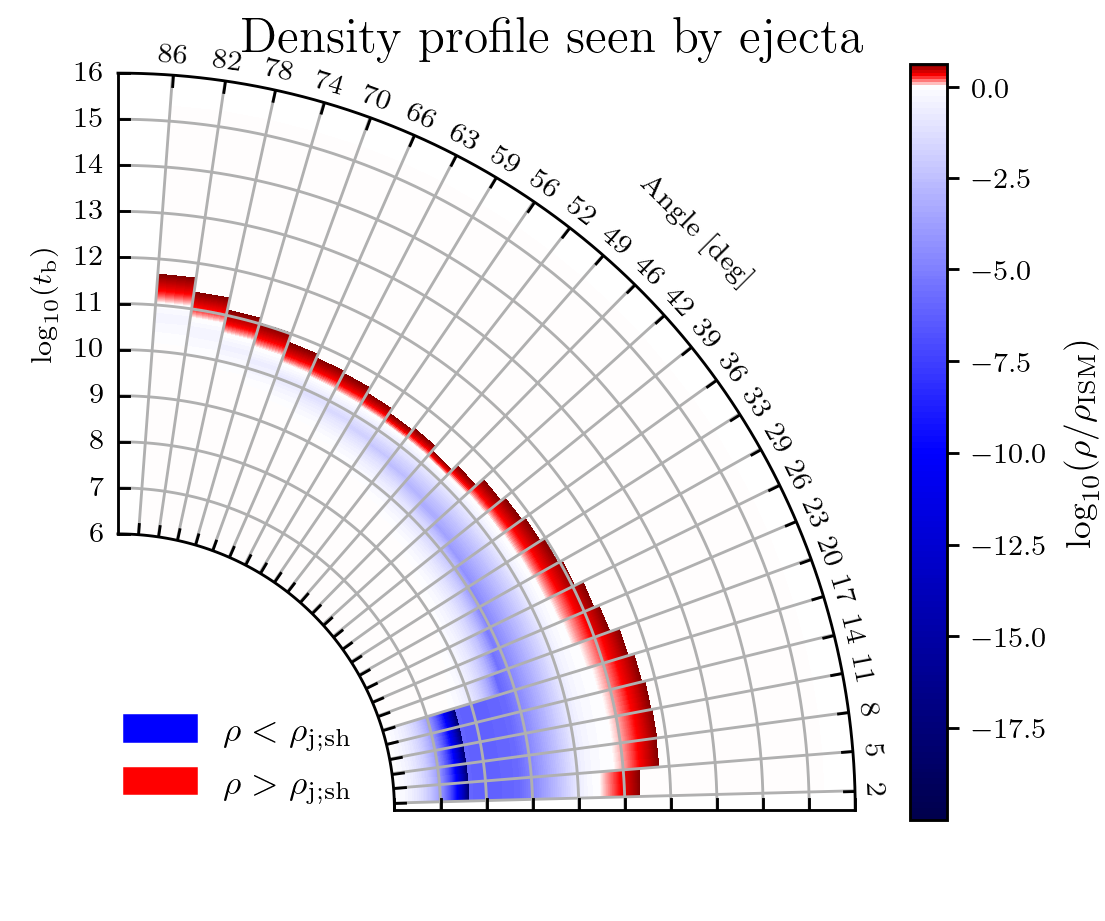
\includegraphics[height=4cm]{figures/bw_ej_dens_ism_evol_fast_shell_2.png}
            }};
        }
        \uncover<1->{ % <-> |
            \node (img1) [anchor=center,scale=1,opacity=1] at ([shift={(10.cm,1.7cm)}]current page.center){
                \parbox{1.0\textwidth}{
                    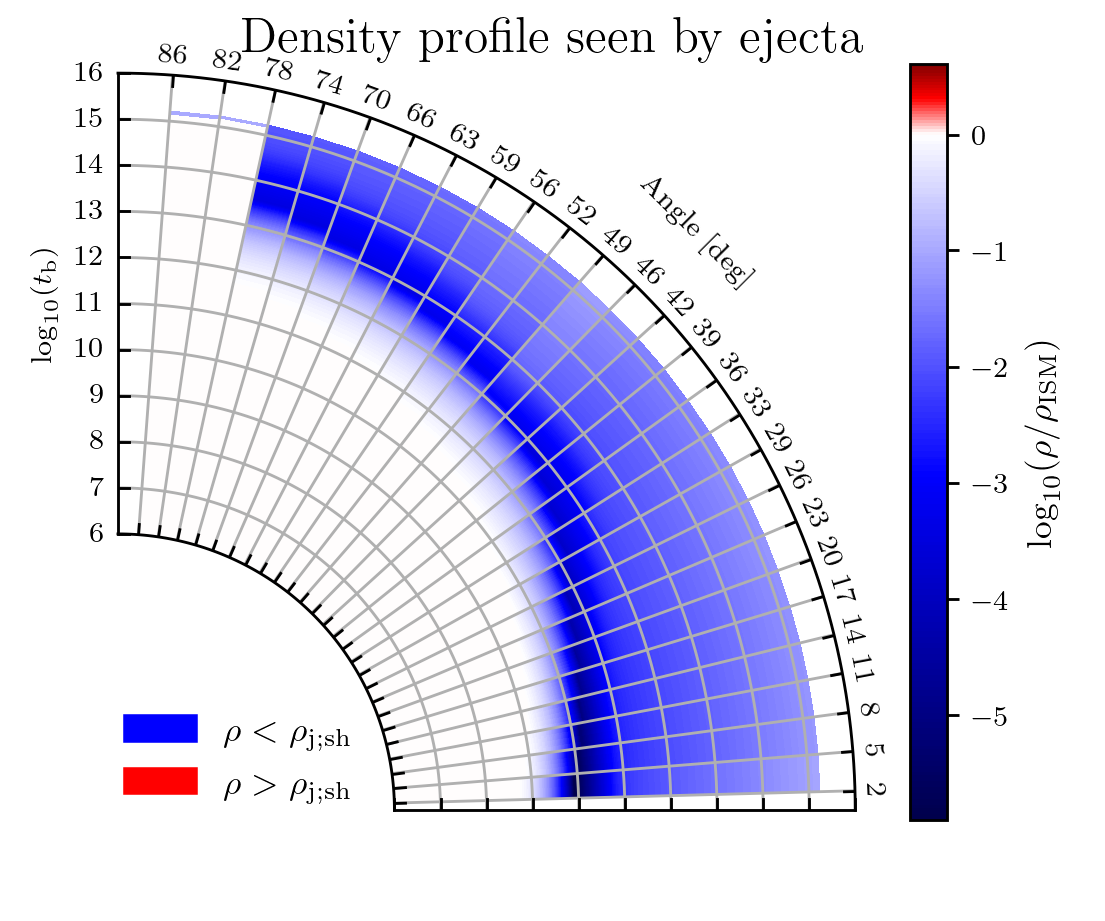
\includegraphics[height=4cm]{figures/bw_ej_dens_ism_evol_slow_shell.png}
            }};
        }
        \uncover<1->{ % <-> |
            \node (img1) [anchor=center,scale=1,opacity=1] at ([shift={(10.cm,-2.3cm)}]current page.center){
                \parbox{1.0\textwidth}{
                    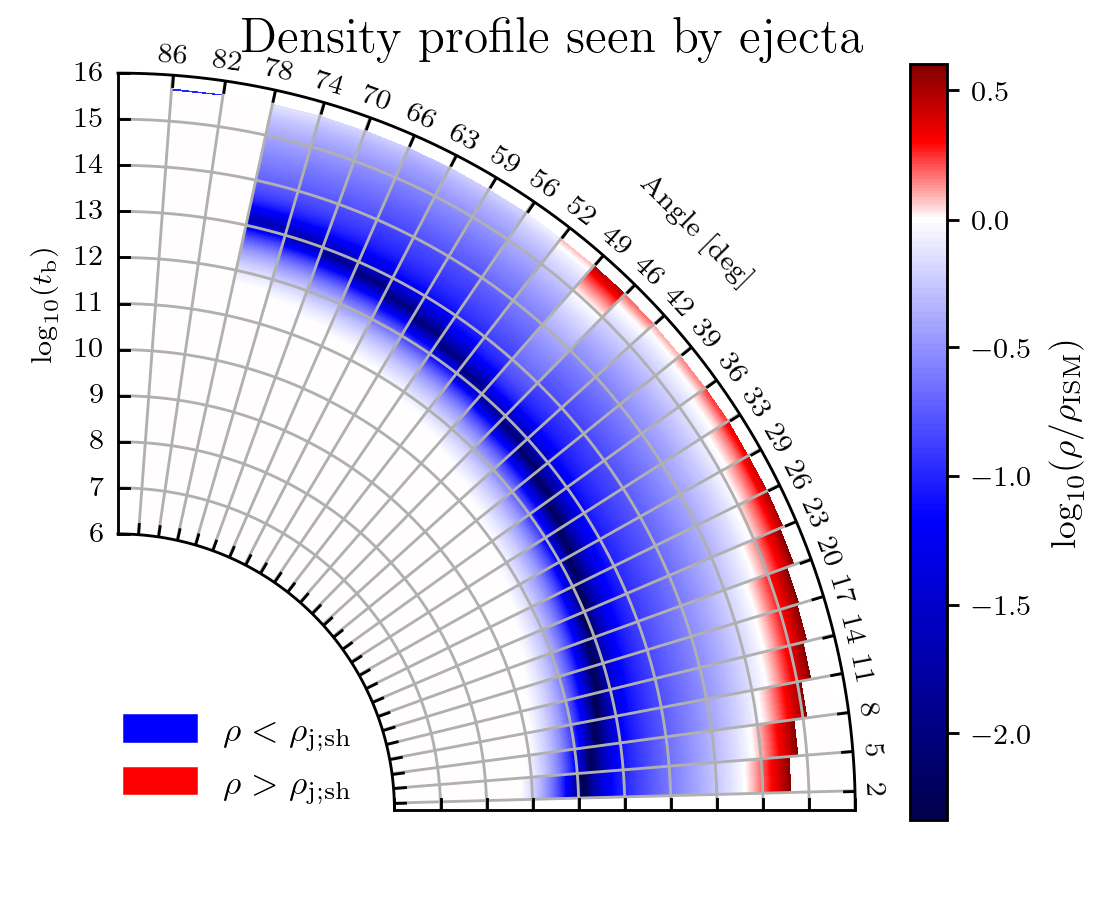
\includegraphics[height=4cm]{figures/bw_ej_dens_ism_evol_fast_shell.png}
            }};
        }
    \end{tikzpicture}
\end{frame}

% =============================================================================================

\subsection{Sky Images}
\begin{frame}{}  %% ---------- Intro/motivation 
    \begin{tikzpicture}[overlay,remember picture]
        \uncover<1->{ % <-> |
            \node (t1) [anchor=center,scale=1,opacity=1] at ([shift={(-4.5cm,1.2cm)}]current page.center){
                \parbox{0.45\textwidth}{
                    Sky image: 
                    
                    for the jet shows the motion of the flux centroid -- constraining inclanation
                    For the ejecta traces its angular deistribution (\textcolor{red}{if resolved})
                    
                    Further investigations required! 
                    
                    Is it possible to observe with very-long-base-line interferometers?
            }};
        }
        \uncover<1->{ % <-> |
            \node (img1) [anchor=center,scale=1,opacity=1] at ([shift={(6.cm,1.7cm)}]current page.center){
                \parbox{1.0\textwidth}{
                    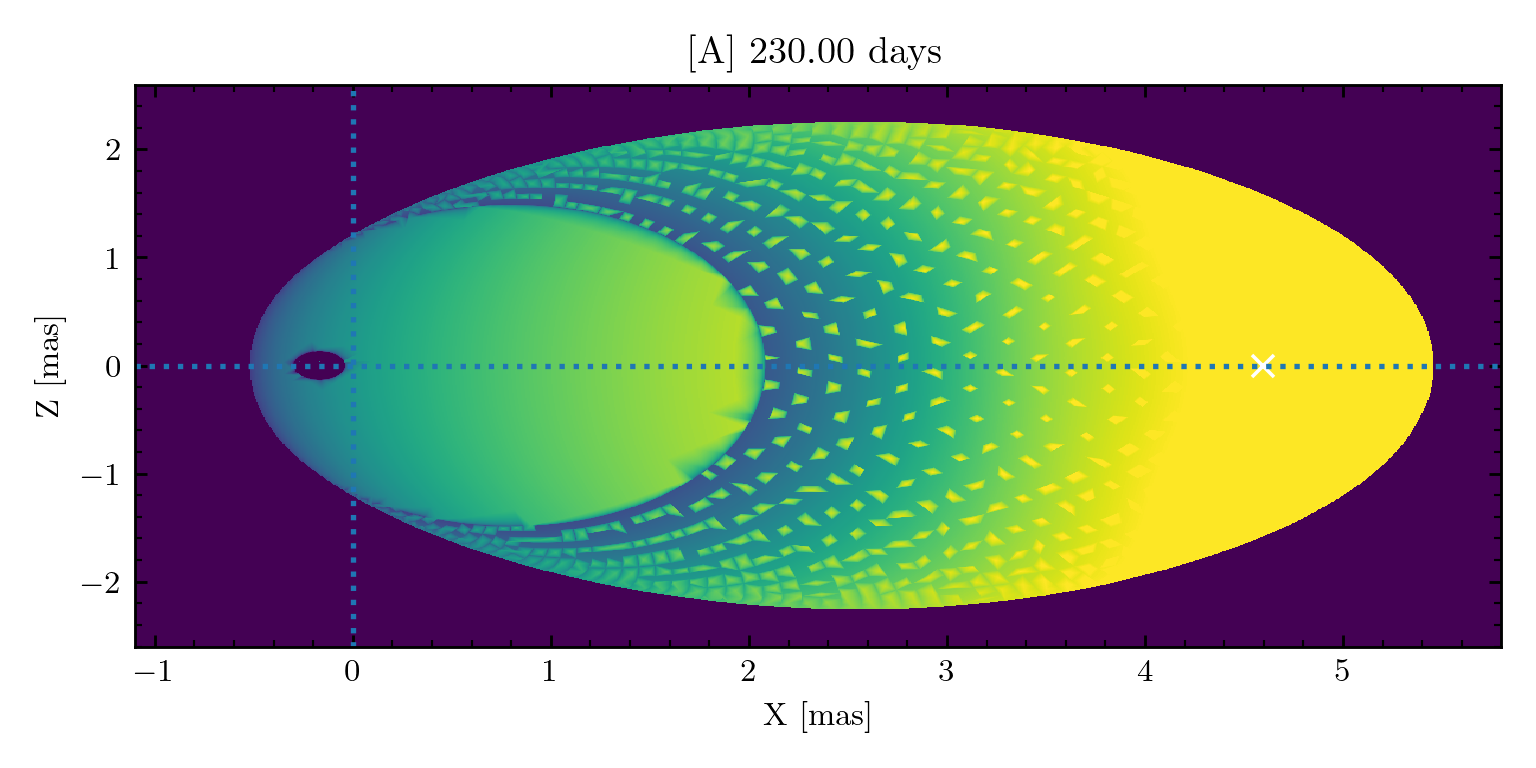
\includegraphics[height=4cm]{figures/plot_sky_image_jet.png}
            }};
        }
        \uncover<1->{ % <-> |
        \node (img1) [anchor=center,scale=1,opacity=1] at ([shift={(6.cm,-2.3cm)}]current page.center){
            \parbox{1.0\textwidth}{
                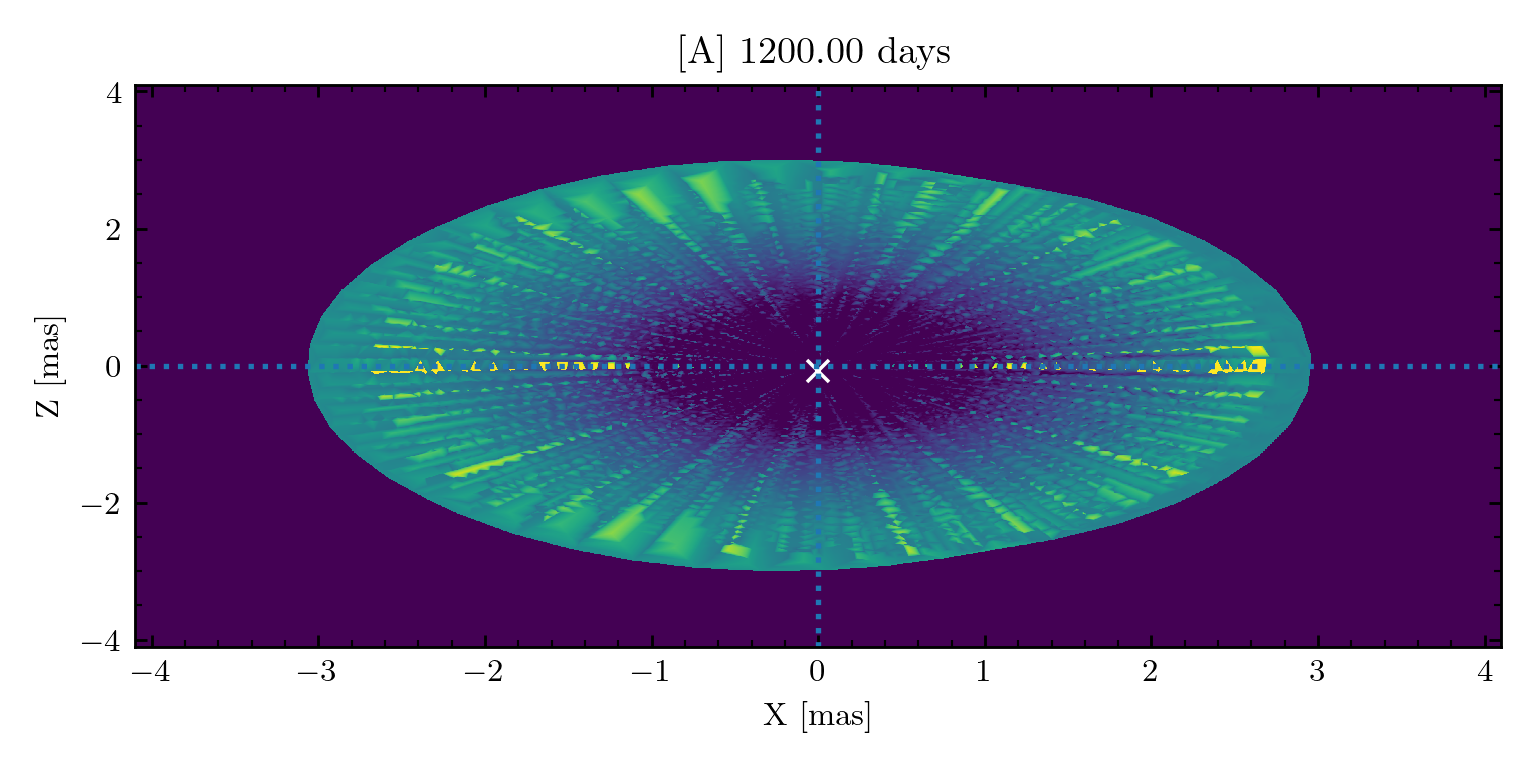
\includegraphics[height=4cm]{figures/plot_sky_image_ejecta.png}
        }};
        }
    \end{tikzpicture}
\end{frame}